 \documentclass{beamer}[10]

\usepackage{graphicx}
\usepackage{xcolor}
\usepackage{tabto}
%\usepackage{beamerthemesplit}
\usepackage{tikz}
\usepackage{cancel}
\usepackage{verbatim}
\usepackage{fancybox}
\usepackage{enumerate}
\usepackage{amsmath,amssymb,amsthm,textcomp,mathtools}
\usepackage[super]{nth}
\usepackage[amssymb]{SIunits}
\usepackage{booktabs}
\usepackage{cancel}
\usepackage{bm}
\usepackage[utf8]{inputenc}
\usepackage{tabularx}
\usepackage{ragged2e}
\newcolumntype{Y}{ >{\RaggedRight\arraybackslash}X}
\usetikzlibrary{arrows,shapes}
\newcommand\T{\rule{0pt}{2.6ex}}
\newcommand\B{\rule[-1.2ex]{0pt}{0pt}}
\definecolor{UUcrimson}{RGB}{204,0,0}
\mode<presentation>
{ \usetheme{default}
  \usecolortheme[named=UUcrimson]{structure}
  \useinnertheme{circles}
  \setbeamercovered{transparent}
  \setbeamertemplate{blocks}[rounded]
  \usefonttheme[onlymath]{serif}
  \setbeamertemplate{navigation symbols}{}
  \setbeamertemplate{footline}[page number]
  \setbeamertemplate{navigation symbols}{}
  \setbeamercolor{section in toc}{fg=black,bg=white}
  \setbeamercolor{alerted text}{fg=UUcrimson!80!gray}
  \setbeamercolor*{palette primary}{fg=white,bg=UUcrimson}
  \setbeamercolor*{palette secondary}{fg=UUcrimson!70!black,bg=gray!15!white}
  \setbeamercolor*{palette tertiary}{bg=UUcrimson!80!black,fg=gray!10!white}
  \setbeamercolor*{palette quaternary}{fg=UUcrimson,bg=gray!5!white}
  \setbeamercolor*{palette sidebar primary}{fg=UUcrimson!10!black}
  \setbeamercolor*{palette sidebar secondary}{fg=white}
  \setbeamercolor*{palette sidebar tertiary}{fg=UUcrimson!50!black}
  \setbeamercolor*{palette sidebar quaternary}{fg=gray!10!white}
  \setbeamercolor{titlelike}{parent=palette primary,fg=white}
  \setbeamercolor{frametitle}{bg=UUcrimson}
  \setbeamercolor{frametitle right}{bg=UUcrimson}
  \setbeamercolor*{separation line}{}
  \setbeamercolor*{fine separation line}{}
}

\usetikzlibrary{backgrounds}
\makeatletter
\tikzstyle{every picture}+=[remember picture]
\tikzset{%
  fancy quotes/.style={
    text width=\fq@width pt,
    align=justify,
    inner sep=1em,
    anchor=north west,
    minimum width=\linewidth,
    font=\itshape
  },
  fancy quotes width/.initial={.8\linewidth},
  fancy quotes marks/.style={
    scale=8,
    text=white,
    inner sep=0pt,
  },
  fancy quotes opening/.style={
    fancy quotes marks,
  },
  fancy quotes closing/.style={
    fancy quotes marks,
  },
  fancy quotes background/.style={
    show background rectangle,
    inner frame xsep=0pt,
    background rectangle/.style={
      fill=gray!25,
      rounded corners,
    },
  }
}
\newenvironment{fancyquotes}[1][]{%
\noindent
\tikzpicture[fancy quotes background]
\node[fancy quotes opening,anchor=north west] (fq@ul) at (0,0) {``};
\tikz@scan@one@point\pgfutil@firstofone(fq@ul.east)
\pgfmathsetmacro{\fq@width}{\linewidth - 2*\pgf@x}
\node[fancy quotes,#1] (fq@txt) at (fq@ul.north west) \bgroup}
{\egroup;
\node[overlay,fancy quotes closing,anchor=east] at (fq@txt.south east) {''};
\endtikzpicture}
\makeatother

\usepackage{scalerel}[2014/03/10]
\usepackage{stackengine}
\usepackage{empheq}
\newcommand*\widefbox[1]{\fbox{\hspace{0.5em}#1\hspace{0.5em}}}

\newcommand\reallywidetilde[1]{\ThisStyle{%
  \setbox0=\hbox{$\SavedStyle#1$}%
  \stackengine{-.1\LMpt}{$\SavedStyle#1$}{%
    \stretchto{\scaleto{\SavedStyle\mkern.2mu\sim}{.5467\wd0}}{.4\ht0}%
%    .2mu is the kern imbalance when clipping white space
%    .5467++++ is \ht/[kerned \wd] aspect ratio for \sim glyph
  }{O}{c}{F}{T}{S}%
}}
\usepackage{media9}

\logo{
\includegraphics[width=0.75cm]{logo.jpg}}
\author[Gibbs]{Dr. Jeremy A. Gibbs}
\institute{Department of Mechanical Engineering\\University of Utah}
\date{Fall 2016}
\title{LES of Turbulent Flows: Lecture 18}
\begin{document}

%----------------------------------------------------------------------------------------
%	TITLE & TOC SLIDES
%----------------------------------------------------------------------------------------

\begin{frame} 
  \titlepage
\end{frame}

%------------------------------------------------

\begin{frame}
\frametitle{Overview}
\tableofcontents
\end{frame}

%------------------------------------------------
\section{Evaluating Simulations and SGS Models} %
%------------------------------------------------
\begin{frame}{Evaluating Simulations and SGS Models}
\begin{itemize}
	\item How do we go about testing our models?
	\item How should models be validated and compared to each other?
\end{itemize}
\end{frame}
%------------------------------------------------
\begin{frame}{Evaluating Simulations and SGS Models}
Pope (2004) gives 5 criteria for evaluating SGS models
\begin{itemize}
	\item Level of description in the SGS model
	\item Completeness of the model
	\item The cost and ease of use of the model
	\item The range and applicability of the model
	\item The accuracy of the model
\end{itemize}
Most of these criteria are related to the accuracy of simulation results
\end{frame}
%------------------------------------------------
\begin{frame}{Evaluating Simulations and SGS Models}
\textbf{Accuracy}
\begin{itemize}
	\item Ability of the model to reproduce DNS, experimental, or theoretical statistical features of a given test flow (or the ability to converge to these values with increasing resolution)
\end{itemize}
\end{frame}
%------------------------------------------------
\begin{frame}{Evaluating Simulations and SGS Models}
\textbf{Accuracy}
\begin{itemize}
	\item An important aspect of this is \textbf{grid convergence of simulation statistics}. 
	\item This is not always done, but is an important aspect of simulation validation. 
	\item Note that this convergence (especially in high-Re flows) may not be exact, we may only see approximate convergence.
\end{itemize}
\end{frame}
%------------------------------------------------
\begin{frame}{Evaluating Simulations and SGS Models}
\textbf{Cost}
\begin{itemize}
	\item When examining the above, it is important to include the cost of each model (and comparisons between alternative models)
	\item One model may give better results at a lower grid resolution (larger $\Delta$) but include costs that are excessive
\end{itemize}
\end{frame}
%------------------------------------------------
\begin{frame}{Evaluating Simulations and SGS Models}
\textbf{Cost}
\begin{itemize}
	\item Example: Scale-dependent Lagrangian dynamic model (Stoll and Port\'{e}-Agel, 2006)
	\item 38\% increase in cost over constant Smagorinsky model
	\item 15\% increase over plane averaged scale-dependent model
	\item How much of a resolution increase can we get in each direction for a 30\% cost increase?? Only a little more than 3\% in each direction!
\end{itemize}
\end{frame}
%------------------------------------------------
\begin{frame}{Evaluating Simulations and SGS Models}
\textbf{Completeness}
\begin{itemize}
	\item  A ``complete'' LES and SGS model would be one that can handle different flows with simply different specification of BCs, initial conditions, and forcings
	\item In general LES models are not complete due to grid requirements and (possibly) ad hoc tuning for different flows
\end{itemize}
\end{frame}
%------------------------------------------------
\begin{frame}{Evaluating Simulations and SGS Models}
\textbf{Completeness}
\begin{itemize}
	\item  Example from RANS: mixing length models are \underline{incomplete} (different flow different $\ell$) 
	\item Meanwhile, the $k$-$\epsilon$ model can be thought of as \underline{complete} for RANS since it can be applied to any flow
\end{itemize}
\end{frame}
%------------------------------------------------
\begin{frame}{Test Case: Turbulent Boundary Layers}
An example from Guerts (2004) of the effect of different SGS models on boundary layer development 
\begin{figure}
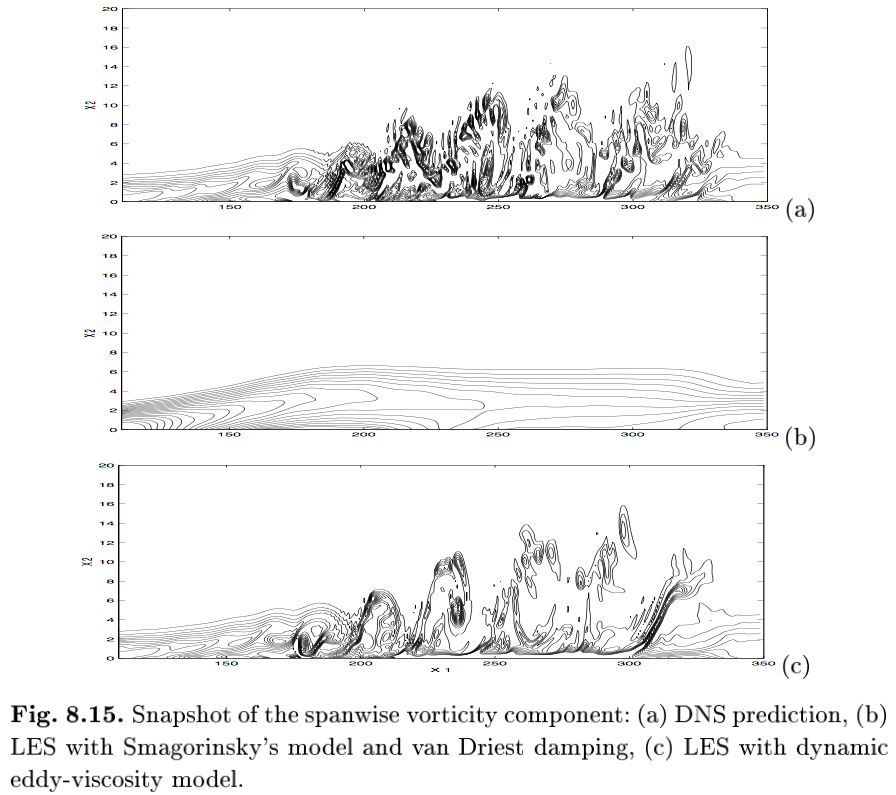
\includegraphics[width=0.75\textwidth]{compare1}	
\end{figure}

\end{frame}

%------------------------------------------------
\begin{frame}{Test Case: Stable Boundary Layers}
An example from GABLS3 (Gibbs, unpublished)
\begin{figure}
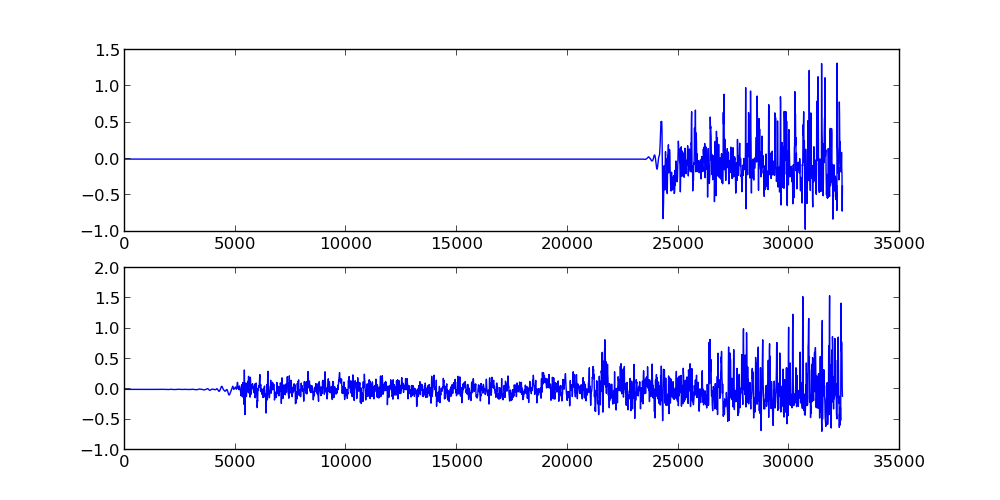
\includegraphics[width=0.85\textwidth]{compare23}
~\\Near-surface vertical velocity fluctuations as produced by OULES with the Smagorinsky (top) and Deardorff (bottom) SGS models
\end{figure}

\end{frame}

%------------------------------------------------
\begin{frame}{Test Case: Backward Facing Step}
An example from Cabot and Moin (1999) 
\begin{figure}
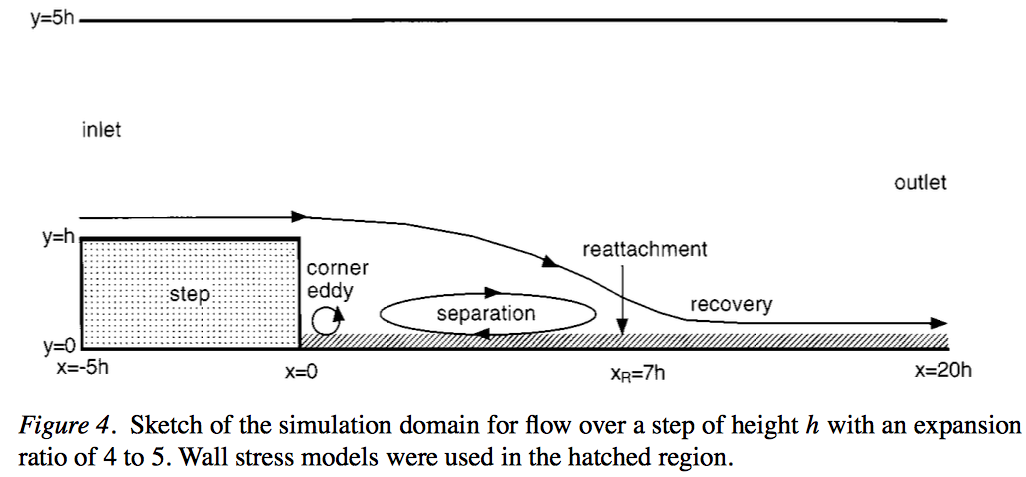
\includegraphics[width=0.85\textwidth]{compare2}	
\end{figure}

\end{frame}

%------------------------------------------------
\begin{frame}{Test Case: Backward Facing Step}
An example from Cabot and Moin (1999) 
\begin{figure}
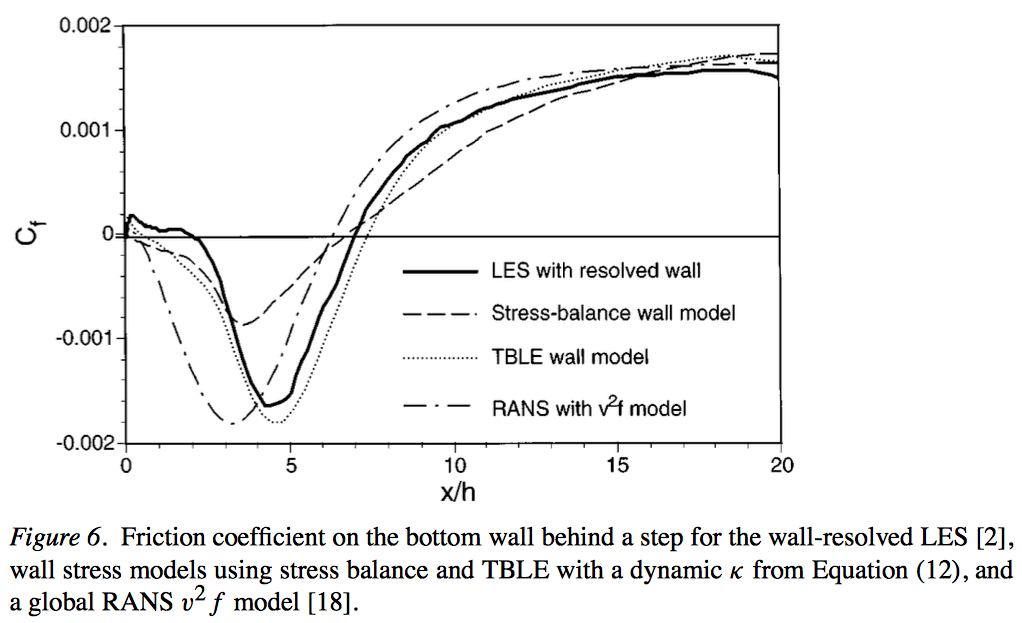
\includegraphics[width=0.85\textwidth]{compare3}	
\end{figure}
\end{frame}

%------------------------------------------------
\begin{frame}{Test Case: Backward Facing Step}
An example from Cabot and Moin (1999) 
\begin{figure}
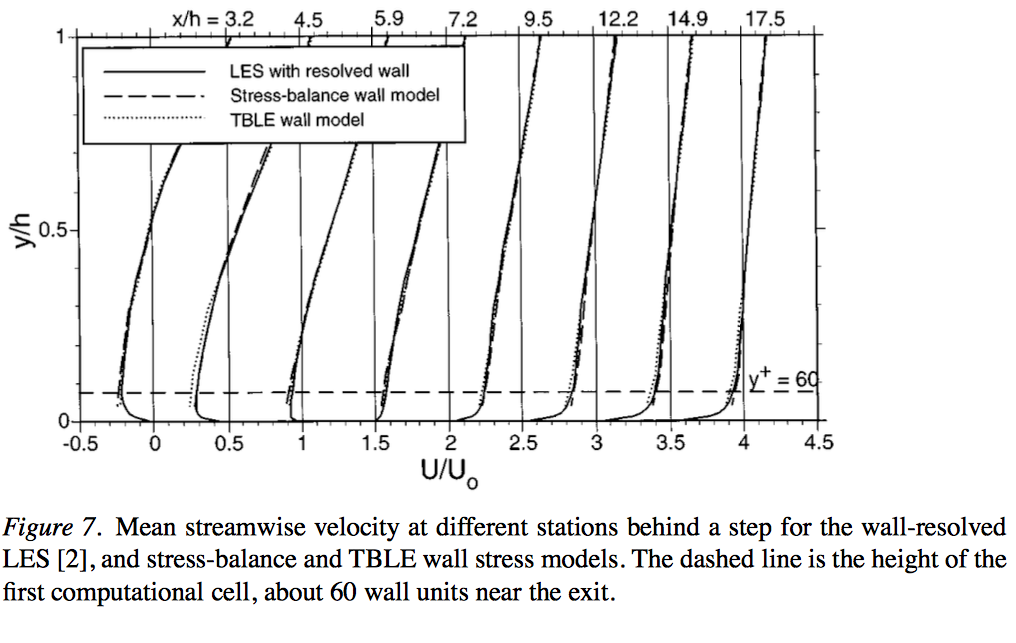
\includegraphics[width=0.85\textwidth]{compare4}	
\end{figure}

\end{frame}

%------------------------------------------------
\begin{frame}{Test Case: Mixing Layer}
An example from Geurts (2004)
\begin{center}
  \begin{tabular}{ c | c | c }\hline\hline
    \textbf{Name} & \textbf{Model for $\tau_ij$} & \textbf{Plot legend} \\ \hline\hline
    M0 & No model & $-$ \\
    M1 & Smagorinsky & $\star$ \\
    M2 & Similarity & $\times$ \\
    M3 & Nonlinear & $+$ \\
    M4 & Dynamic Smagorinsky & $--$ \\
    M5 & Dynamic Mixed & $\ldots$ \\
    M6 & Dynamic Nonlinear & $-\cdot$ \\
    \hline\hline
  \end{tabular}
\end{center}
\end{frame}

%------------------------------------------------
\begin{frame}{Test Case: Mixing Layer}
An example from Geurts (2004)
\begin{figure}
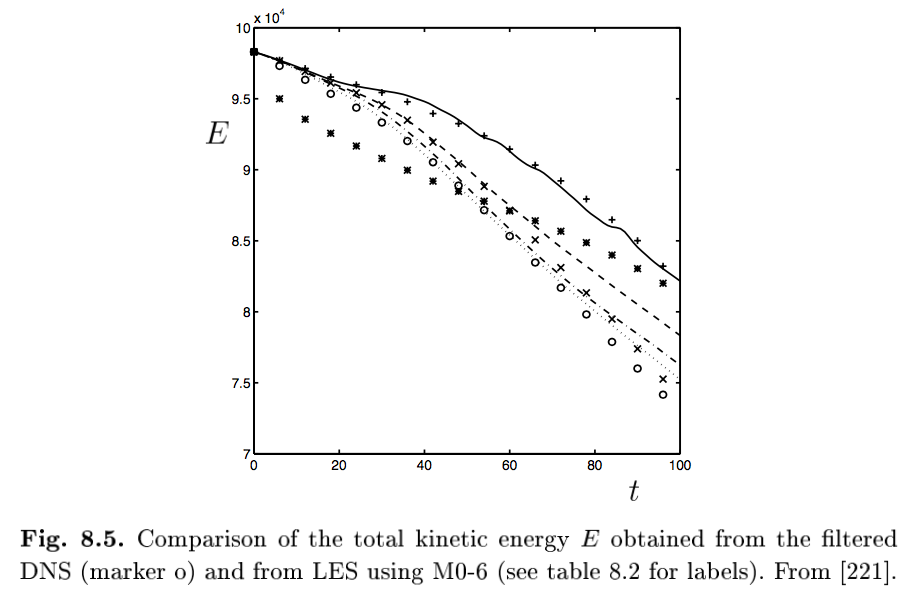
\includegraphics[width=0.85\textwidth]{compare5}	
\end{figure}
\end{frame}
%------------------------------------------------
\begin{frame}{Test Case: Mixing Layer}
An example from Geurts (2004)
\begin{figure}
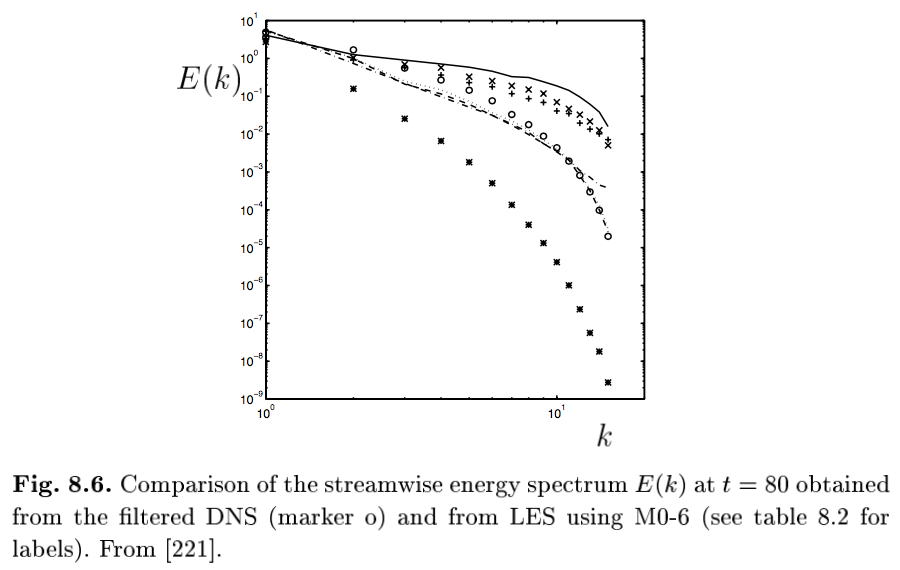
\includegraphics[width=0.85\textwidth]{compare6}	
\end{figure}
\end{frame}
%------------------------------------------------
\begin{frame}{Test Case: Mixing Layer}
An example from Geurts (2004)
\begin{figure}
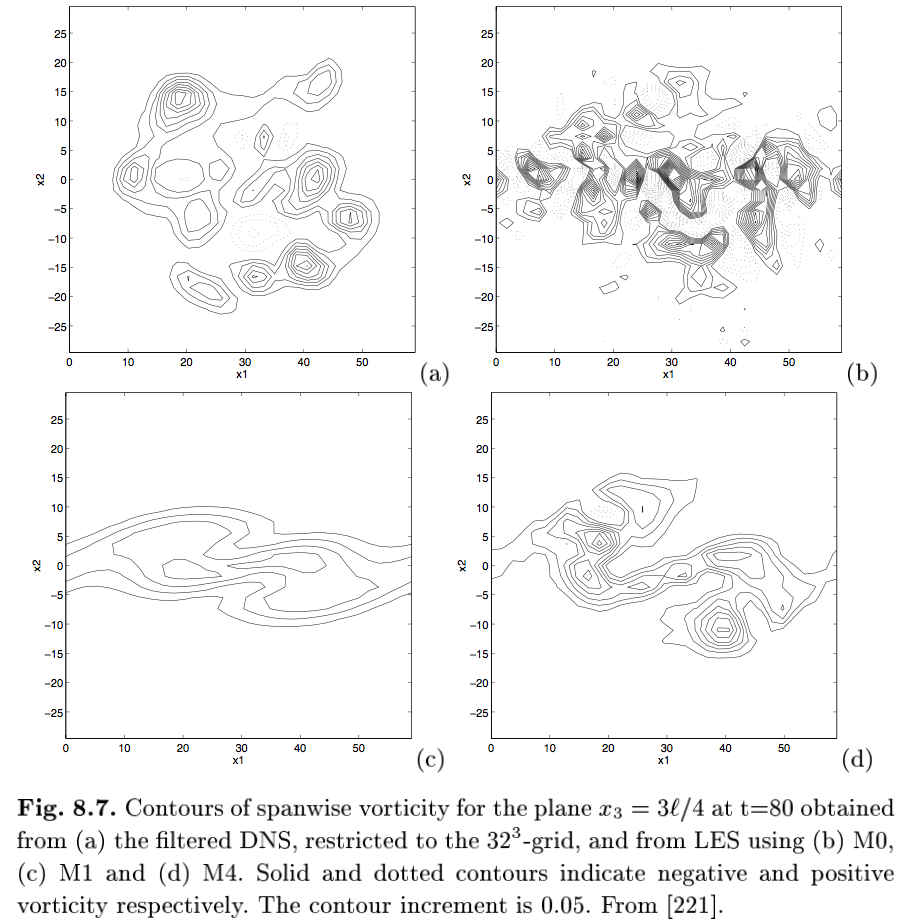
\includegraphics[width=0.685\textwidth]{compare7}	
\end{figure}
\end{frame}

%------------------------------------------------
\begin{frame}{Accuracy of LES Models}
%\begin{itemize}
%	\item Here we will look at some examples of different measurements of simulation accuracy and evaluation, as well as a few common test cases for LES
%\end{itemize}
\begin{columns}[T]
    \begin{column}{.45\textwidth}
    \begin{minipage}[c][0.85\textheight][c]{\linewidth}
    \begin{itemize}
	\item An example of the accuracy of LES models to predict flow statistics (from Port\'{e}-Agel et al 2000 and  Andren et al. 1994)
	\item $\Phi$ is non-dimensional velocity gradient
	\item In panel (a), Dashed line: traditional Smagorinsky model with $C_0 = 0.1$ and $n = 2$; dot-dashed line: traditional Smagorinsky model with $C_0 = 0.17$ and $n = 1$; solid line: standard dynamic model
\end{itemize}
      \end{minipage}
    \end{column}
    \begin{column}{.5\textwidth}
      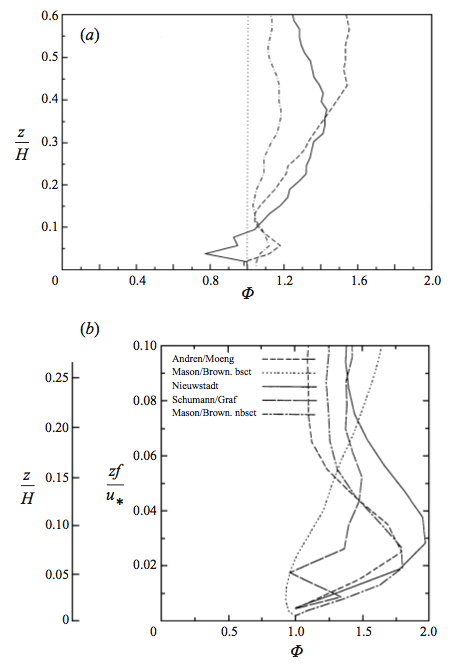
\includegraphics[width=\textwidth]{compare8}
    \end{column}
  \end{columns}
\end{frame}

%------------------------------------------------
\begin{frame}{Accuracy of LES Models}
An example of the accuracy of LES models to predict flow statistics (from Port\'{e}-Agel et al 2000)
\begin{figure}
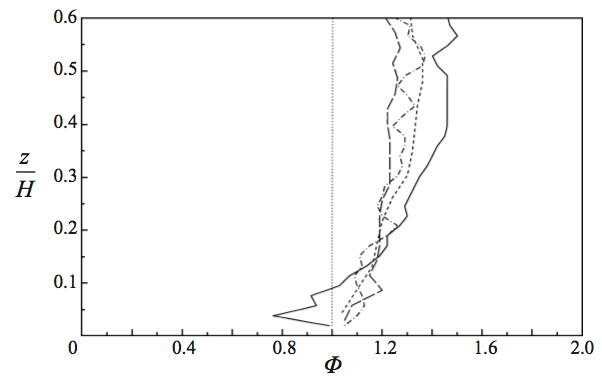
\includegraphics[width=0.8\textwidth]{compare9}
~\\Non-dimensional velocity gradient 
\end{figure}
\end{frame}

%------------------------------------------------
\begin{frame}{Accuracy of LES Models}
An example of the accuracy of LES models to predict flow statistics (from Port\'{e}-Agel et al 2000)
\begin{figure}
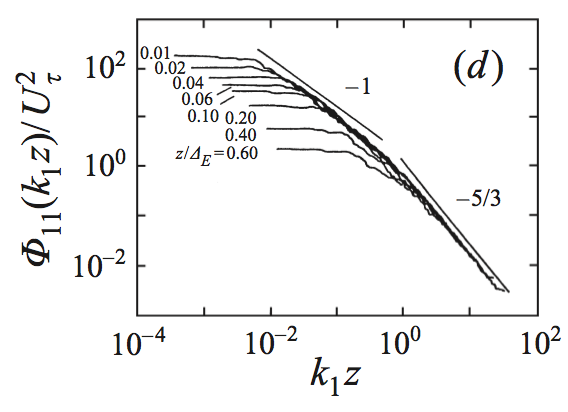
\includegraphics[width=0.49\textwidth]{compare10}
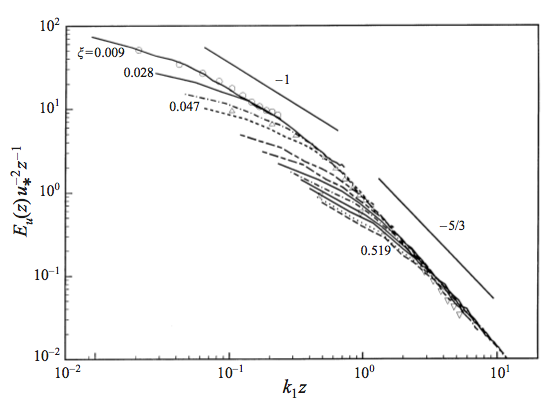
\includegraphics[width=0.51\textwidth]{compare11}
~\\left: Streamwise velocity spectra from Perry et al (1986)\\right: Streamwise velocity spectra at two  different resolutions 
\end{figure}
\end{frame}

%------------------------------------------------
\begin{frame}{Test Case: Isotropic Turbulence LES}
An example from Lu et al (2008) 
\begin{figure}
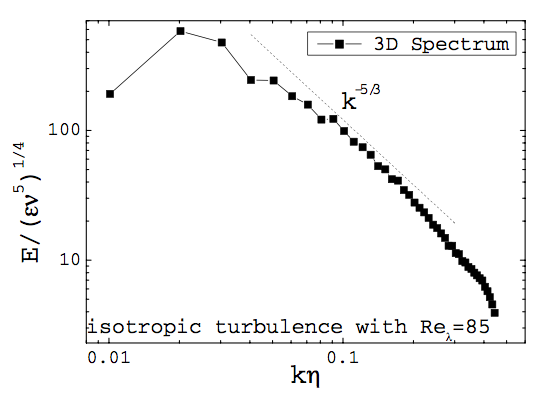
\includegraphics[width=0.5\textwidth]{compare12}
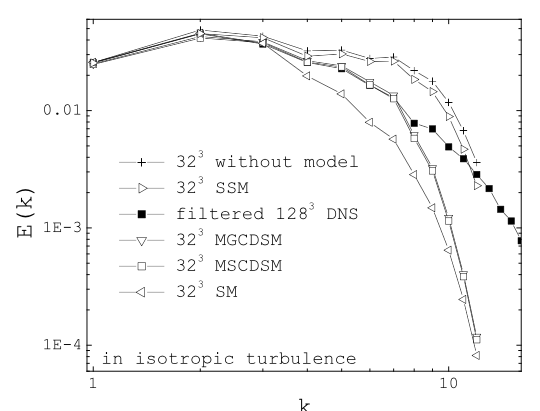
\includegraphics[width=0.5\textwidth]{compare13}
~\\left: velocity spectra from DNS\\right: velocity spectra from filtered DNS and LES
\end{figure}
\end{frame}

%------------------------------------------------
\begin{frame}{Test Case: Isotropic Turbulence LES}
An example from Lu et al (2008) 
\begin{figure}
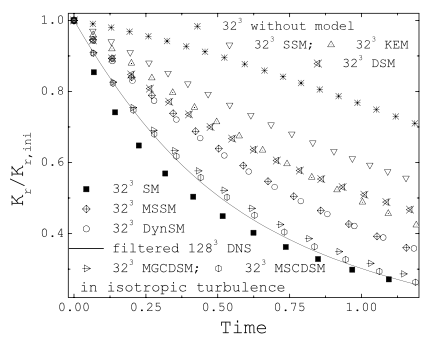
\includegraphics[width=0.8\textwidth]{compare14}
~\\energy decay
\end{figure}
\end{frame}

%------------------------------------------------
\begin{frame}{Test Case: Flow Over a 2D Hill}
An example from Wan et al (2007) 
\begin{figure}
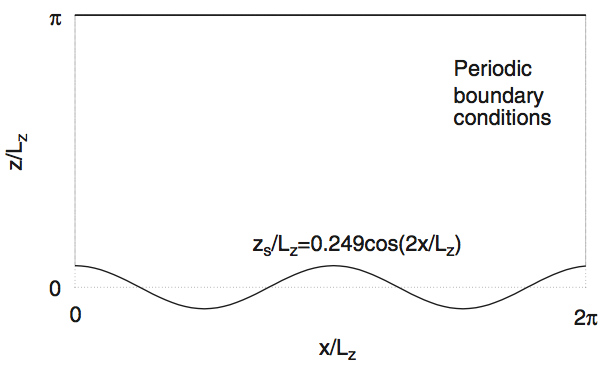
\includegraphics[width=0.8\textwidth]{compare15}
\end{figure}
\end{frame}

%------------------------------------------------
\begin{frame}{Test Case: Flow Over a 2D Hill}
An example from Wan et al (2007) 
\begin{figure}
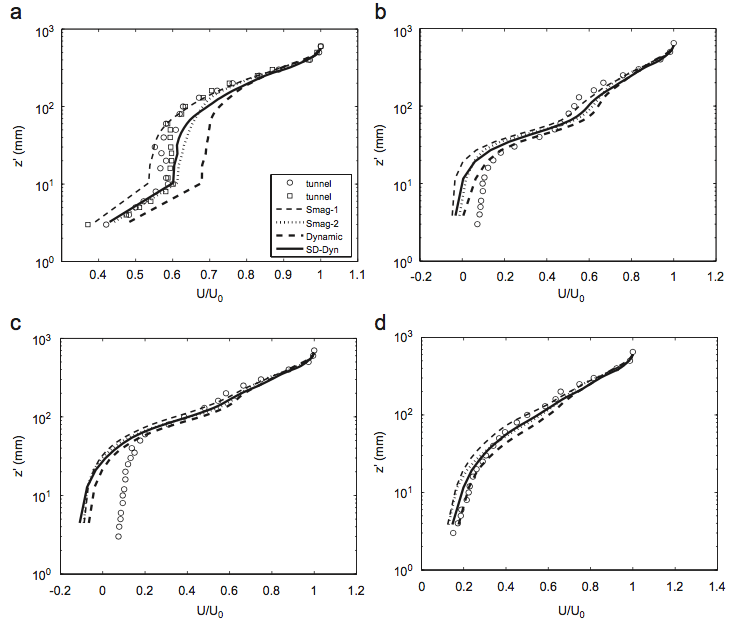
\includegraphics[width=0.7\textwidth]{compare16}
~\\ Velocity comparison with data and different models
\end{figure}
\end{frame}
%------------------------------------------------
\begin{frame}{Test Case: Flow Over a 2D Hill}
An example from Wan et al (2007) 
\begin{figure}
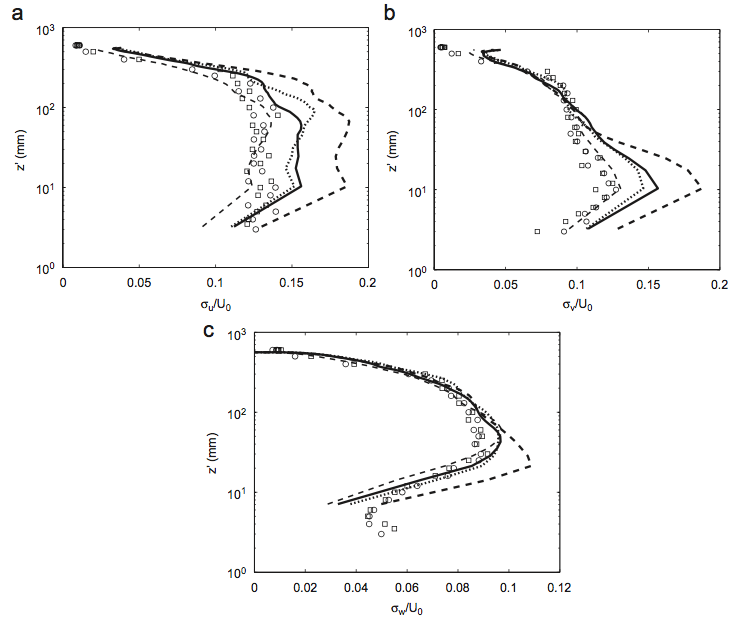
\includegraphics[width=0.7\textwidth]{compare17}
~\\ Velocity comparison with data and different models
\end{figure}
\end{frame}
%------------------------------------------------
\begin{frame}{Example: Grid Resolution}
An example from Sullivan and Patton (2011) 
\begin{itemize}
	\item  Re-examined a typical flow used in atmospheric simulations as an analog for daytime conditions (high-Re, weakly sheared convection)
	\item Goal: understand mesh dependence of a particular SGS model (Deardorff 1980 type, 1-equation) 
\end{itemize}
\end{frame}

%------------------------------------------------
\begin{frame}{Example: Grid Resolution}
An example from Sullivan and Patton (2011)
\begin{itemize}
	\item Domain: $5120 \times 5120 \times 2048$ m$^3 (x,y,z)$ 
\end{itemize}
\begin{center}
  \begin{tabular}{ c | c | c | c}\hline\hline
    \textbf{Run} & \textbf{Grid points} & $(\Delta x, \Delta y, \Delta z) [m]$ & $\Delta_f [m]$\\ \hline\hline
    A & $32^3$ & (160, 160, 64) & 154 \\
    B & $64^3$ & (80,80,32) & 77.2 \\
    C & $128^3$ & (40,40,16) & 38.6 \\
    D & $256^3$ & (20,20,8) & 19.3\\
    E & $51263$ & (10,10,4) & 9.6 \\
    F & $1024^3$ & (5,5,2) & 4.8 \\
    \hline\hline
  \end{tabular}
\end{center}
\end{frame}
%------------------------------------------------
\begin{frame}{Example: Grid Resolution}
An example from Sullivan and Patton (2011) 
\begin{figure}
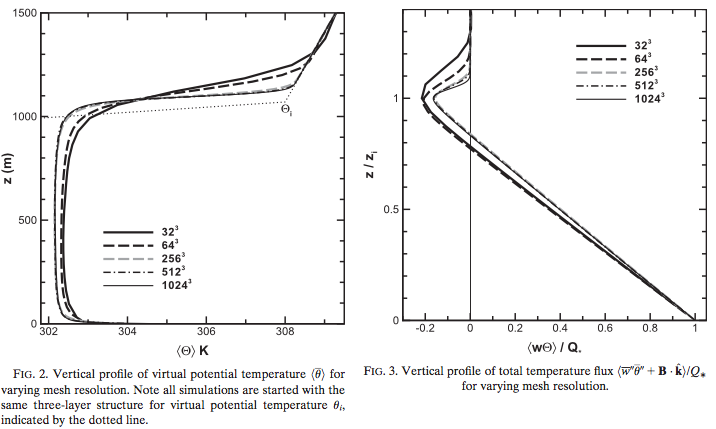
\includegraphics[width=1\textwidth]{compare18}
\end{figure}
\end{frame}
%------------------------------------------------
\begin{frame}{Example: Grid Resolution}
An example from Sullivan and Patton (2011) 
\begin{figure}
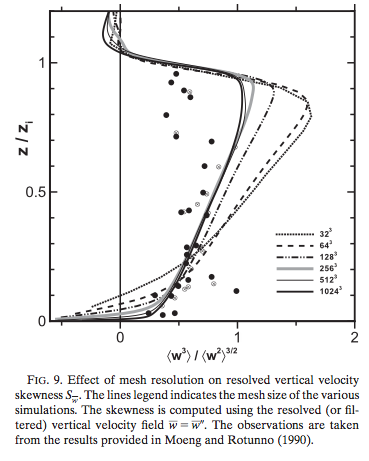
\includegraphics[width=0.55\textwidth]{compare19}
\end{figure}
\end{frame}

%------------------------------------------------
\begin{frame}{Example: Grid Resolution}
An example from Sullivan and Patton (2011) 
\begin{figure}
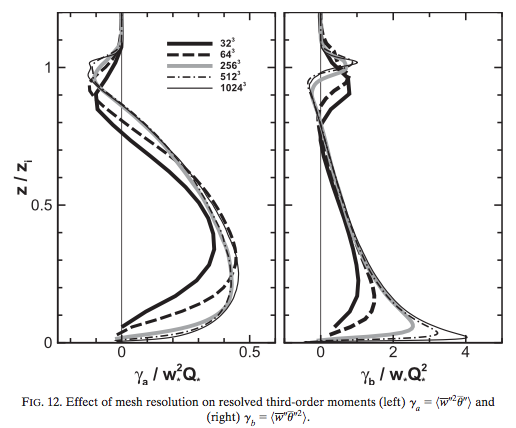
\includegraphics[width=0.8\textwidth]{compare20}
\end{figure}
\end{frame}
%------------------------------------------------
\begin{frame}{Example: Grid Size}
An example from Gibbs, Fedorovich, van Heerwarden (unpublished)
\begin{figure}
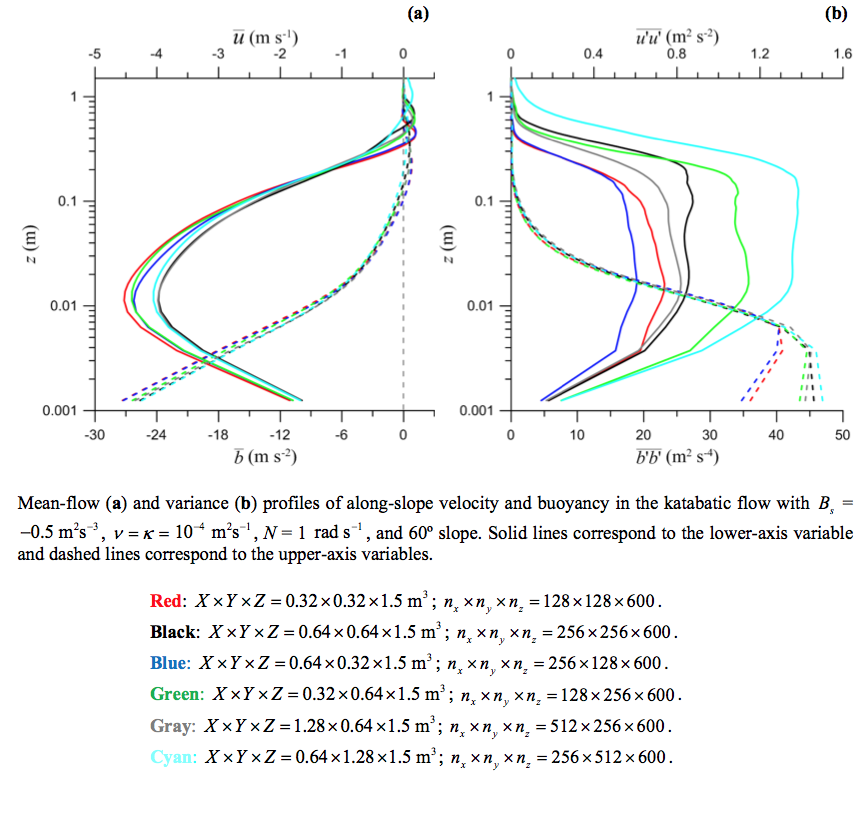
\includegraphics[width=0.8\textwidth]{compare21}
\end{figure}
\end{frame}
%------------------------------------------------
\begin{frame}{Example: Grid Size}
An example from Gibbs, Fedorovich, van Heerwarden (unpublished)
\begin{figure}
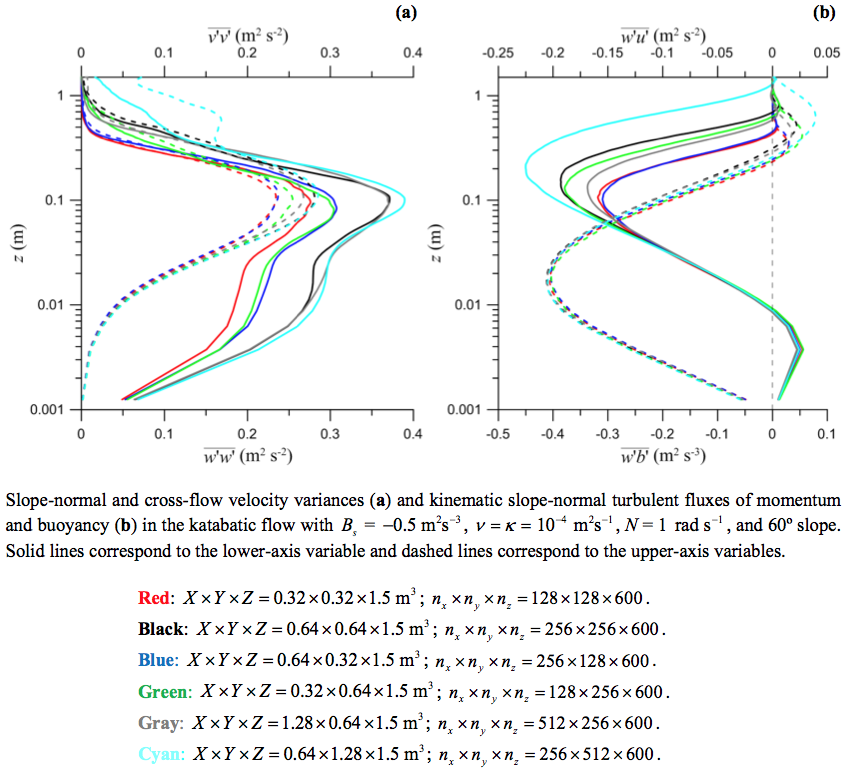
\includegraphics[width=0.8\textwidth]{compare22}
\end{figure}
\end{frame}



%------------------------------------------------


\end{document}

